\vspace{-2mm}

\section{Experiment}
\label{sec:experiment}
\subsection{Experimental Setup}
\textbf{Dataset Configurations}. The experiments are performed on WorldScope benchmark comprising 5,000 examples in total, with 4,500 examples for training and 500 for testing. All models will be tested on the same test split with \emph{three assessment forms} (SCQ, MCQ, and TFQ), and instantiated via prompt templates for \emph{three modality inputs} (textual, numerical, and visual).

\textbf{Comparison Models}. To provide sufficient experimental evidence for subsequent argumentation under protocal in ~\ref{protocol}, we will test with SOTA LLMs of various modalities on the same backbone families before and after fine-tuning, while taking traditional architecture models as the capability boundary of passive data-fitting method. The full experiment details including model list, input formatting, training, and hyperparameters) are given in Appendix ~\ref{sec:training-protocol}.


\subsection{Main Result and Analysis}
\label{phenomenon}

Table ~\ref{tab:main_results_hierarchical} presents a comprehensive performance comparison across textual, numerical, and visual modalities, encompassing general-purpose LLMs alongside the capability boundary of the passive data-fitting method presented by task-specific traditional-architecture models. The empirical data intuitively reveals several highly counter-intuitive phenomena exhibited by these SOTA LLMs confronting complex physical world representations.

1) \textbf{The Inverse Scaling Phenomenon.}
Contemporary AI development relies heavily on \emph{Scaling Laws}, which posit that model capabilities scale monotonically with parameter count. 
However, our experimental results reveal a counter-intuitive "inverse scaling" phenomenon. 
In the numerical modality, Llama-3.1 (70B) and Mistral-Small-3 (24B) yield MCQ accuracies of 6.40\% and 5.80\%, respectively. 
Not only are these performances inferior to the significantly smaller Vicuna-1.5-7B (MCQ: 12.40\%), but they are also comprehensively dominated by a simple CNN architecture with a mere 0.40M parameters (MCQ: 23.80\%) by a margin of over three times. 
Similarly, in the visual modality, the 90B-parameter Llama-3.2-Vision falls far behind the 4.34M-parameter EfficientNet-B0. 
This stark contrast—where million-parameter networks absolutely suppress hundred-billion-parameter LLMs—intuitively demonstrates that when confronting specific structural regularities of the physical world, merely \emph{scaling up parameters} results in computational redundancy rather than the emergence of \emph{genuine problem-solving capabilities}.

2) \textbf{Hallucination and Fragility of LLMs.}
The Mean and Standard Deviation reported in the table reflects not only the absolute performance but also directly exposes the \emph{stability and epistemic certainty} of the model outputs.
It can be observed that general LLMs are pervasively accompanied by exceptionally high standard deviations across various physical tasks. 
For instance, Llama-3.1 70B scores 54.21\% ± 8.67\% on the numerical TFQ task, and Claude-4.6-opus even reaches 56.36\% ± 8.92\%. 
In contrast, lightweight models (e.g., ResNet-18, EfficientNet-B0) consistently exhibit not only higher means but also significantly lower variances (e.g., EfficientNet-B0 achieving 63.11\% ± 1.85\% on visual TFQ).
Such \emph{drastic performance fluctuations}with standard deviations reaching 8-9 percentage points directly expose the extreme \emph{Logical Fragility} underlying these LLMs. 
In this case, their representational outputs are highly susceptible to random noise in the input context or minor perturbations in the prompt, essentially degenerating into severe hallucination and random guessing. 
% This proves that architectures equipped with appropriate inductive biases can formulate robust and deterministic reasoning logic when addressing physical tasks.

\begin{figure}[!t]
	\centering
	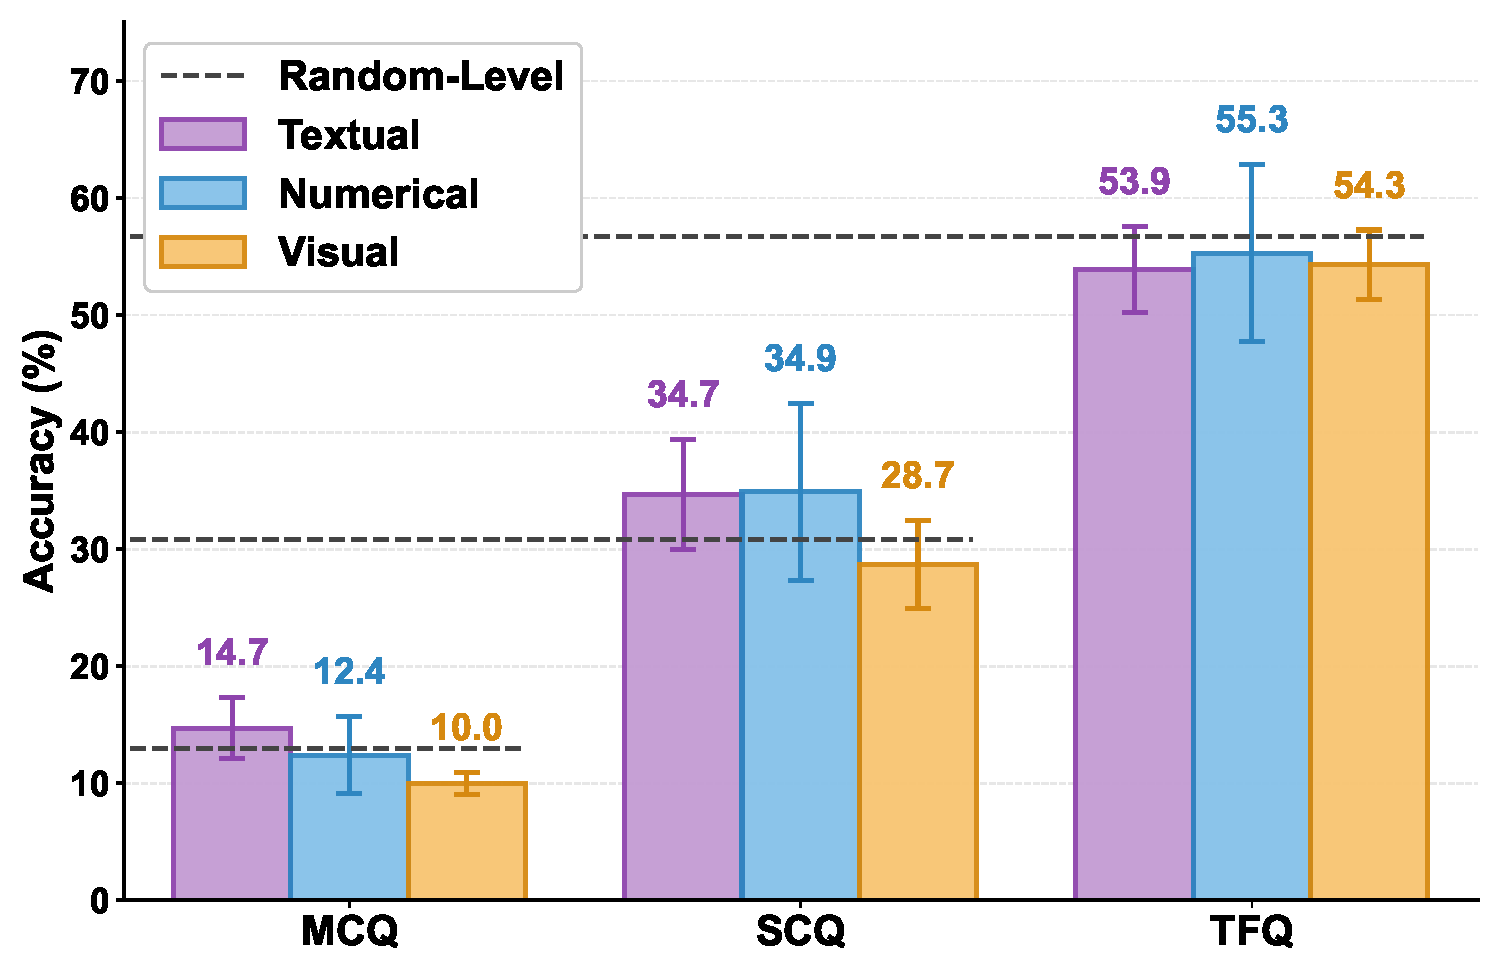
\includegraphics[width=\linewidth]{figure/figure20.pdf}
    \vspace{-5mm}
	\caption{Modality-Agnostic properties along with different models and different problem tasks.}
	\label{fig:cross-modality}
    \vspace{-5mm}
\end{figure}

\subsection{Insight of Capability Collapse}
\label{analysis}
1) \textbf{Complete performance crash.} 
It is widely accepted that the models we tested have represented the capability upper bound of current LLMs.
By contrast, GPT-5.4 scores a mere 8.60\% on MCQ, 26.80\% on SCQ, and 52.02\% on TFQ in the visual modality—falling strictly below the pure random guessing threshold across all three metrics.
Claude-4.6-opus exhibits a similarly dismal and comprehensive collapse (MCQ: 11.40\%, SCQ: 30.60\%, TFQ: 56.59\%).
Therefore, this perceived "ceiling" is now facing a \emph{catastrophic failure} under our evaluation framework across all task formats.
These empirical evidences reveal that these apex models would even fail to reach the mathematical upper probability of random chance, regardless of problem tasks.

2) \textbf{Incompatibility between architecture and physical world.}
More crucially, even within their native and most proficient textual modality, the performance of these top-tier models still remains fundamentally constrained. 
While GPT-5.4 and Claude-4.6-opus barely manage to cross the random baseline on textual MCQ and SCQ, they persistently fall below the baseline on TFQ (e.g., GPT-5.4: 54.23\%, Claude-4.6-opus: 53.54\%). 
Furthermore, they are comprehensively outperformed by the traditional lightweight LSTM architecture across the entire metric matrix (MCQ: 20.00\%, SCQ: 37.20\%, TFQ: 61.74\%).
This persistent cross-modal degradation intuitively proves that the capability collapse of LLMs on heterogeneous physical world tasks is not an accidental byproduct of format complexity or insufficient training.
On the contrary, it exposes that the entire \emph{autoregressive next-token prediction paradigm} itself inherently possesses an \emph{insurmountable capability ceiling}.


